\chapter{Preliminaries}\label{ch:preliminaries}
In the following we present the control system currently used at DLR, the hardware used with it and the software out-of-the-shelf we have used in the development of our algorithm. We also present the reliability problem we have tried to solve with the above-mentioned algorithm. 
\section{Interactive Myocontrol}\label{sec:interactivemyocontrol}
It is the control system currently used at DLR, it provides a graphical interface for the training and management of the different machine learned controller for different kind of prosthetic hands. For our work we have used the machine learned controller based on the method Ridge Regression with Random Fourier Features (RR-RFF), which we have presented in section \ref{sec:ML}. Given the scope of our work we have decided to use, instead a real prosthetic hand, a virtual model of a prosthetic hand which, when connected with Interactive Myocontrol, reproduce accurately the movement signaled by the controller.
\begin{figure}[ht]
    \centering
    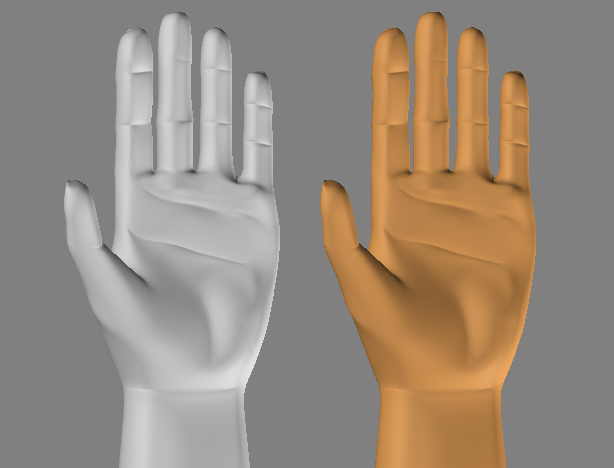
\includegraphics[width=0.5\textwidth]{Images/Blender.PNG}
    \caption{Virtual model of a prosthetic hand used with Interactive Myocontrol. The gray hand is used to reproduce the reference signals, whereas the orange hand is used to reproduce the predictions.}
    \label{fig:hand-blender}
\end{figure}
The hardware used to generate the sEMG signals from the muscular activation of human participants is the Myo Armband manufactured by Thalmic Labs (\href{https://www.thalmic.com}{https://www.thalmic.com}), is provided with eight sEMG sensors uniformly distributed along the bracelet.
\begin{figure}[ht]
    \centering
    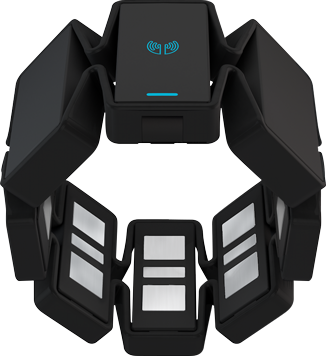
\includegraphics[width=0.5\textwidth]{Images/myo_armband.png}
    \caption{Myo Armband manufactured by \href{https://www.myo.com/techspecs}{Thalmic Labs}}
    \label{fig:myo_armband}
\end{figure}
The sEMG signals produced by the bracelet are the only input signal used by our machine learned controller, before being passed as input to the controller the signals are rectified and mildly low-pass filtered with a 2nd order Butterworth filter (cutoff 1Hz).
The outputs of the machine learned controller are nine different value which corresponds to the activation level of the nine different degrees of freedom (DOFs) of the prosthetic hand. In a real prosthetic hand these nine values are used to directly control the actuators which permits the movement of the hand, whereas in our case these values are used to control the position of the virtual model of the hand. Interactive Myocontrol use the different values of the nine DOFs to define 17 different action that are used as references in the training of the controller. In this work we are only interested in four of these actions, which are: rest, power grasp, wrist flexion and wrist extension; for convenience's sake we will consider as outputs the activation level of the above mentioned actions.
Interactive Myocontrol let the user decide which subset of the 17 actions desires to use in the training of the machine learned controller.
Therefore each sample of the training set $S$ is composed of an input sample $\mathbf{x}_i \in \mathbb{R}^8$ and a corresponding target value $\mathbf{y}_i \in \mathbb{R}^9$. In particular, given the physical limits of the sEMG sensors, each features of the input samples is limited between 0 and 5, therefore we can further limit the input space to $[0, 5]^8$.
As is customary in the current state of the art (see, eg., \cite{hahne2015concurrent}, \cite{sierra2013realistic}) in practice $S$ is built by gathering for each action of interest a certain number of observations while the participant is doing that particular action; each observation is then coupled with the target value associated to the action.
For example, the participant is asked to power grasp ("make a fist"); once the experimenter verifies that the signals have reached a stable pattern, well distinct from the baseline, a suitable number of observations is recorded and associated to (synthetic) target values denoting maximal activation of all fingers. This methodology is called on-off goal-directed training.
Interactive Myocontrol permits an incremental training of the machine learned controller: it is possible for the user to add new training samples after the initial training session and retrain the learning machine using also the new data; in \cite{Strazzulla2017} such machine learned controller is called \textit{Incremental-Learning Myoelectric Controller}
\section{dReal}\label{sec:dReal}
In this work we needed an SMT solver which could manage trascendent functions, due to the utilization of the Random Fourier Features as feature map in the machine learned controller. We chose dReal \cite{gao2013dreal} because it satisfied our requirements and was provided with an API python which could be easily used in our code. It was out of the scope of this thesis to compare the performance of different SMT solver, therefore we didn't consider others than dReal.
In order to handle a wide range of nonlinear real functions dReal implements the framework of $\delta$-complete decision procedures. We say a decision procedures is $\delta$-complete for a set of formulas $S$ if for any $\phi \in S$ the procedure returns \textit{unsat} if $\phi$ is unsatisfiable or \textit{$\delta$-sat} if $\phi^\delta$ is satisfiable.
$\delta$ is an arbitrary positive rational number and $\phi^\delta$ is a syntactic variant of $\phi$ that encodes a notion of numerical perturbation on logic formulas. Essentialy we relax the constrains on the procedure in order to permit answers with an one sided $\delta$-bounded error, therefore $\delta$-complete decision procedures can exploit the power of numerical approximations without losing formal correctness guarantees.